\chapter{绪论}
\section{研究背景}
随着计算机视觉(Computer Vision)
和自然语言处理(Natural Language Processing)技术的迅猛发展,
跨模态智能理解成为人工智能研究的重要方向之一。
其中,视觉问答(Visual Question Answering, VQA)\cite{goyal2017making}任务因其广泛的应用前景和挑战性,
受到了学术界和工业界的广泛关注。例如,给定一幅包含动物的图片,
系统需要能够回答“这只动物是什么颜色?”或“图片中有几只猫?”等问题。
这一任务的核心在于多模态信息的深度融合,即如何在视觉特征和语言信息之间建立有效的联系。
积木世界\cite{hogg1983block}是人工智能研究、教学、实验、评估的重要场景,能够模拟实际应用中物体间的空间关系。
研究积木世界VQA任务,能够有效考察智能体在空间推理方面的能力。
积木世界可通过对不同复杂度的场景的模拟,能够作为范例方便用于大语言模型、自动规划、自然语言处理、模式识别等
不同方向的研究和课程的教学中\cite{chiyahgarcia2024repairsblockworldnew}\cite{silver2023generalizedplanningpddldomains}。
研究积木世界VQA任务,通过不同的积木摆放、堆叠、遮挡等空间布局的积木世界数据,
能够有效地用于研究和考察智能体在空间推理方面的能力\cite{johnson2017clevr}。

多年以来,有多种方法被提出用于解决VQA任务,其中
视觉语言模型(Visual Language Model, VLM)因其强大的多模态理解能力而备受关注。
VLM是一种多模态模型,能够同时处理图像和文本信息,并生成与图像内容相关的自然语言响应。
如图\ref{fig:vlm-example}所示为VLM的一个简单流程示例。
VLM通过将视觉编码器与大语言模型结合,赋予模型“看”与“理解”的能力。与传统的计算机视觉模型不同,VLM 不受固定
类别集或特定任务 (如分类或检测) 约束。在大量文本和图像/视频字幕对的语料上进行重新训练,
VLM 可以用自然语言进行指导,并用于处理许多典型的视觉任务以及新的生成式 AI 任务,
例如摘要和视觉问答。如图\ref{fig:vlm-architecture}所示为VLM的通用架构,包括视觉编码器、投影器和大语言模型(Large Language Model, LLM)三个部分。
视觉编码器(如CLIP模型)具有图像与文本的关联能力,负责提取图像特征。投影器由一组网络层构成,负责将视觉特征转换为LLM可理解的标记(Token)。
LLM负责生成文本输出,支持对话、推理等任务,目前任何现有的LLM(如ChatGPT、LLaMA、DeepSeek等)都可以用来构建VLM。
\begin{figure}
    \centering
    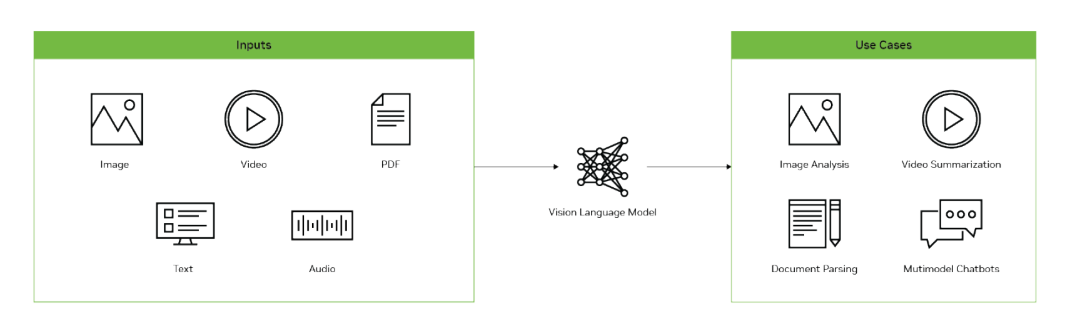
\includegraphics[width=\textwidth]{figures/VLM-example.png}
    \caption{视觉语言模型用例}
    \label{fig:vlm-example}
\end{figure}

\begin{figure}[htb]
    \centering
    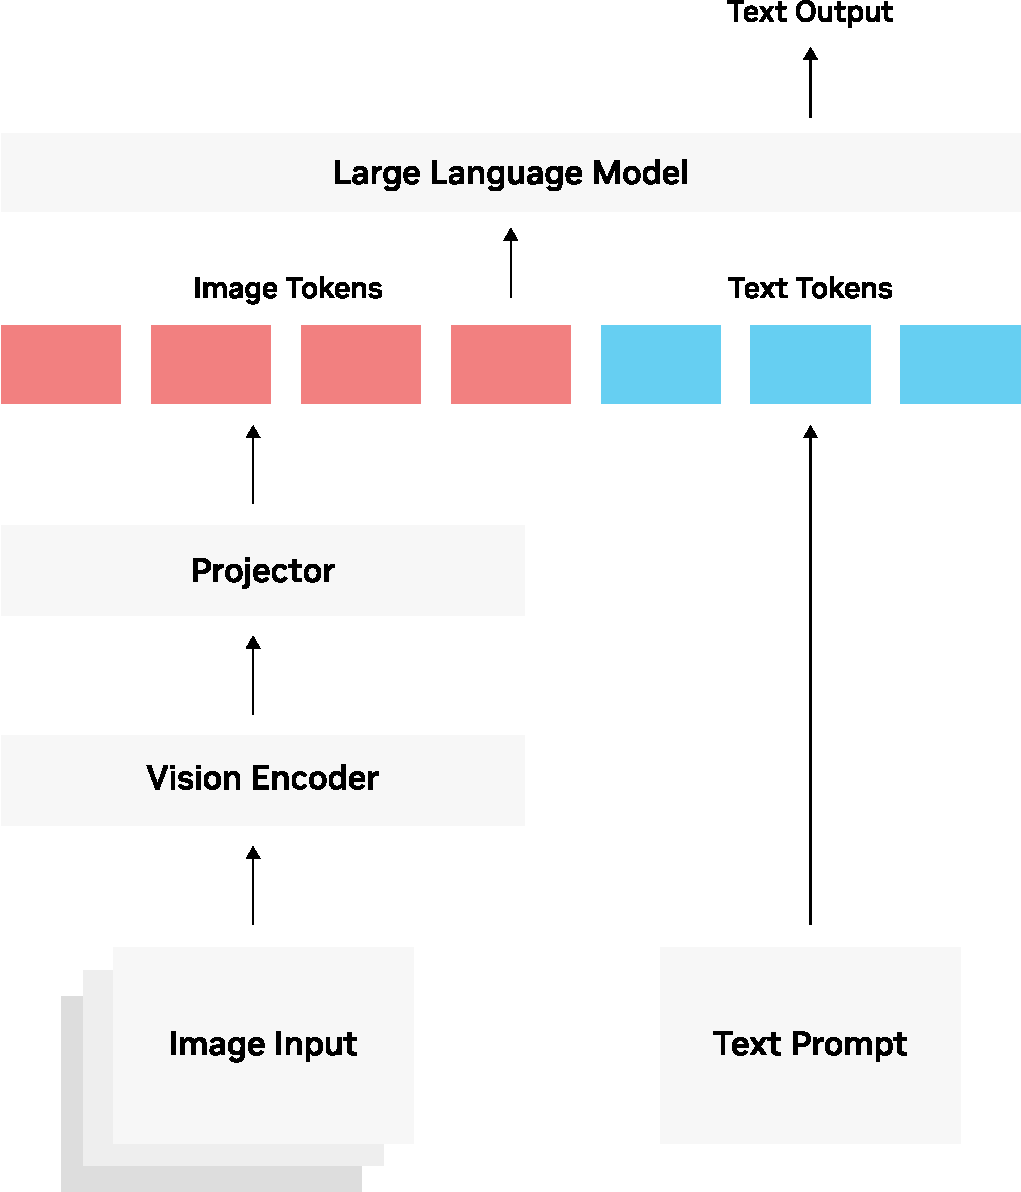
\includegraphics[scale=0.6]{figures/vlm-architecture-diagram-crop.pdf}
    \caption{视觉语言模型的通用三部分架构}
    \label{fig:vlm-architecture}
\end{figure}

尽管VLM在图像分类\cite{pratt2023does}、字幕生成\cite{alaluf2024myvlm}、
目标检测\cite{kuo2022f}、视频理解\cite{huang2024lita}和文档解析\cite{lv2023kosmos}
等各种任务中取得了良好效果,但VLM仍难以有效应对部分可见场景中基于空间推理的VQA任务。
部分可见指的是在图像中,某些物体或其特征由于遮挡、模糊、视野受限、噪声或其他原因而不可见的情况,
导致模型无法从图像中获得解决问题所需的全部信息。
现有的VLM在部分可见场景中解决VQA任务时,可能会出现幻觉\cite{vardi2025clipupclipbasedunanswerableproblem}
、空间关系推理能力下降\cite{chen2024spatialvlmendowingvisionlanguagemodels}\cite{anis2025limitationsvisionlanguagemodelsunderstanding}
,并且在对象识别和计数任务中表现不佳\cite{campbell2024understandinglimitsvisionlanguage},不能真正理解图像信息\cite{rahmanzadehgervi2025visionlanguagemodelsblind}等问题。
这类部分可见场景在现实世界中广泛存在,例如在机器人抓取、自动驾驶、安防监控等实际应用中,
系统往往需要在信息不完全的条件下对场景作出准确理解和决策。

因此,研究能够在部分可见场景中进行准确空间推理的VQA方法,不仅具有理论挑战性,也具有重要的工程价值。
一方面,它有助于提升人工智能系统在复杂环境中的稳健性和泛化能力;
另一方面,也为智能机器人\cite{gao2024physically}\cite{nasiriany2024pivot}、
AR/VR交互系统\cite{konenkov2024vr}等场景中的感知与决策提供了新的技术路径。

为了解决多模态模型在空间推理方面的问题,研究者们提出了一些新的方法。近年来,
神经符号方法(Neuro-Symbolic Methods)得到了广泛关注。在多模态空间推理场景中,
神经符号方法使用深度学习技术进行感知,为输入的图像和问题分别生成符号表示,再使用符号系统进行推理求解,
可以有效提升多模态模型在空间推理方面的能力。

在神经符号方法中,神经网络的选择十分多样,通常包括卷积神经网络(Convolution Neural Network, CNN)、
循环神经网络(Recurrent Neural Network, RNN)及其变体、图神经网络(Graph Neural Network, GNN)和
Transformer架构及LLM。相比其它神经网络,LLM用于神经符号系统,具有以下突出优势:
\begin{enumerate}[itemsep=0pt,parsep=0pt]
    \item 丰富的预训练知识库。LLM在大规模语料上进行预训练,具备广泛的世界知识和语言理解能力,这使得它们在处理涉及常识推理和多领域知识整合时,比专门针对单一任务训练的网络更具优势。
    \item 自然语言理解与生成能力。LLM能够将符号系统产生的抽象逻辑或规则,用自然语言进行解释和反馈,从而降低了人机交互的门槛,并使得系统的推理过程更易于理解和验证。
    \item 零样本/少样本学习能力。由于在大规模数据上学习到了通用的语言模式,LLM在面对新领域或数据较少的任务时,往往能够直接发挥作用,从而提高神经符号系统的泛化能力。
    \item 灵活的上下文建模。LLM能够捕捉长距离依赖和上下文信息,这对于将符号系统中离散的知识点进行有机整合,以及在复杂场景中实现动态推理具有重要意义。
\end{enumerate}
结合以上各项理由,将LLM作为神经符号系统中的神经模块,能够与符号系统形成互补,既利用符号逻辑的严谨性,又发挥神经网络在语义理解和自然语言生成方面的优势,从而构建更强大、更灵活的智能系统。

在神经符号方法中,符号系统的选择同样多种多样,例如知识图谱嵌入(Knowledge Graph Embeddings, KGE)、逻辑神经网络(Logical
 Neural Networks, LNN)都为信息表示和推理提供了新思路。其中,回答集编程(Answer Set Programming,ASP)也被
越来越多地采用作为符号系统。ASP是一种声明式编程范式,可用于解决复杂的人工智能问题,其起源于对逻辑编程、非单调推理和知识表示的研究。
相比其它符号系统,ASP被更多用于神经符号方法中,主要是由于以下几点优势:(1)明确的逻辑语义与可解释性。ASP基于严格定义的逻辑规则,其推理过程透明、易于解释。这一特性在需要精确推理和结果可验证的任务中尤为重要\cite{gelfond1988stable};
(2)强大的非单调推理能力。ASP自然支持非单调逻辑推理,能够处理默认情况和异常情形,这使其在面对现实世界中不完全或动态变化的信息时表现出色\cite{gelfond1988stable};
(3)成熟的求解器与工具支持。像Clingo这样的ASP求解器已经经过长期验证,具有高效、稳定的特点,能够处理大规模问题,这为实际应用提供了有力保障\cite{gebser2012answer};
(4)便于与神经网络等模块整合。ASP的声明式表达方式使其易于与神经网络输出的信息对接,形成互补优势,从而提升整体系统的推理能力\cite{garcez2002neural}。
ASP的这些特性使得它作为符号系统的杰出代表,被广泛应用于神经符号方法中。

尽管神经网络采用了预训练的LLM,而符号系统部分选用了ASP,但将二者有效结合在一起仍然是一项复杂的任务。
为此,近年来出现了一些神经符号框架,试图通过模块化设计和统一接口来简化LLM与ASP的集成开发流程\cite{wang2024dspybasedneuralsymbolicpipelineenhance}。
尽管现有的框架为LLM结合ASP的开发过程提供了诸多便利,降低了使用门槛,然而其在ASP规则的自动拓展方面存在不足,
需要依赖人工干预进行规则扩充,在这一方面仍存在改进空间。

为了测试模型解决空间推理问题的能力,涌现了诸如CLEVR、GQA、COCO等数据集。
这些数据集由问题答案对(Question and Answer Pair,以下简称QA对)组成,
并且包含问题对应的场景图像。CLEVR是一种积木世界的数据集,因其高度结构化的场景构造、精确标注的物体属性及复杂的空间关系,
而被广泛用于人工智能的研究和课堂教学等重要场景。
然而,CLEVR数据集图像均基于完整场景生成,所有回答问题的信息都直接可见,缺乏现实环境中常见的部分可见性,
难以有效考察VLM在部分可见场景中的推理能力\cite{sam-abraham-etal-2024-clevr}。
因此,要考察模型在部分可见积木世界中对空间推理问题的解答能力,需要对CLEVR进行改进,以使其具备部分可见性。

自动规划作为人工智能领域的一个重要分支,其核心目标是让计算机能够像人类一样,自主地制定实现特定目标的行动计划。
对能够完成积木世界中寻找、挪动物体等任务的智能体而言,空间推理显然是其能够完成任务指令的前置要求。
目前,市面上业已出现不少人工智能课程教学的演示系统,然而很少有演示教学系统
关注自动规划课程中的积木世界空间推理,不能展示智能体运用哪些知识以完成空间推理,进而达到最终目标。
为此,设计并实现一个自动规划课堂教学演示原型系统,展示智能体如何在部分可见的积木世界场景下完成空间推理,
对启发学生理解人工智能思考过程,进一步提升自动规划课程教学的可视化水平,具有十分重要的意义。

综上所述,积木世界作为空间推理研究的重要场景,虽在可视化、可控性和评估便利性方面具备显著优势,
但现有视觉语言模型在面对部分可见或遮挡场景时,其空间推理能力仍显不足。
神经符号方法通过引入形式化的逻辑推理机制,有效弥补了深度学习在可解释性和系统性推理方面的短板,
尤其是在复杂空间关系建模中展现出潜力。然而,当前神经符号VQA框架中ASP规则的拓展仍主要依赖于人工,
难以灵活适应动态环境和多样化任务需求。为进一步提升神经符号模型在部分可见场景中的空间推理性能,
亟需构建具挑战性的高质量数据集,并探索规则自动补充机制与大语言模型的协同方式,
从而推动视觉问答系统在积木世界场景中的智能推理能力发展,为自动规划课堂中教师向学生展示智能体如何理解外部环境信息并进行推理提供了便利。
\section{相关研究现状}
基于前述背景,本文的研究目标明确为:提升神经符号方法用于部分可见的积木世界的空间推理问答的准确率。
为达成该研究目标,所需了解的
研究领域包括VQA技术、VQA数据集、ASP程序生成、空间推理、神经符号方法在空间推理中的应用等。为此,本节将对这些领域的相关研究进行综述。
\subsection{VQA技术的研究现状}
VQA是由Antol等人\cite{Antol2015VQA}提出的,是人工智能领域中一个富有挑战性的交叉研究方向,
涉及计算机视觉(CV)、自然语言处理(NLP)和机器学习(ML)等多个学科。
其核心任务是让机器能够根据给定的图像内容和相关的自然语言问题,生成准确的自然语言答案。
VQA不仅要求模型理解图像中的视觉信息(如物体、属性、关系)和问题的语义意图,还需要进行复杂的推理,
融合这两种模态的信息来找到或生成答案。近年来,随着深度学习技术的发展,VQA领域取得了显著进展,但也面临着诸多挑战。

早期的VQA模型通常采用相对简单的框架,例如使用卷积神经网络(CNN)提取图像特征,使用循环神经网络(RNN)
或长短期记忆网络(LSTM)编码问题,然后通过简单的融合策略(如元素积、拼接)结合两种模态的特征,最后输入到一个分类器中预测答案。

然而,这类方法难以有效关联问题中的关键信息和图像中的特定区域。为了解决这个问题,注意力机制
被广泛引入VQA模型中。其核心思想是让模型根据问题的指导,动态地聚焦于图像中最相关的区域。其中, Anderson等人提出的自下而上的注意力机制\cite{anderson2018bottom}
成为后续许多模型的基础。该方法首先使用Faster R-CNN等目标检测器提取图像中的显著区域,
然后根据问题生成一个查询向量,计算该查询与各个区域特征的相似度(注意力权重),最后对区域特征进行加权求和,
得到与问题高度相关的视觉特征。这种方法显著提升了模型性能,因为它能更精确地定位与问题相关的视觉证据。
后续研究进一步发展了注意力机制,如分层注意力\cite{lu2016hierarchical}和共同注意力,后者允许模型同时学习图像区域和问题词语之间的相互关联,从而实现更深层次的跨模态信息交互。

随着Transformer架构在NLP领域的巨大成功,研究者们也开始将其应用于VQA任务,以更好地捕捉长距离依赖和模态间的复杂交互。
这些模型通常利用Transformer的自注意力和交叉注意力机制。ViLBERT\cite{lu2019vilbert}和 LXMERT\cite{tan2019lxmert}是早期的代表性模型。
它们采用双流架构,分别处理视觉和文本输入,并通过跨模态Transformer层进行信息交互和融合。VL-BERT\cite{su2019vl}和 Oscar\cite{li2020oscar}则采用了单流架构,
将图像区域特征和文本词嵌入拼接在一起,输入到一个统一的Transformer编码器中进行联合建模。Oscar还引入了目标标签作为“锚点”,
连接图像区域和对应的文本描述,增强了跨模态对齐。

这些基于Transformer的视觉语言预训练(Vision-Language Pre-training, VLP)模型通常在大规模的图像-文本对数据上进行预训练,
学习通用的跨模态表示,然后在特定的VQA数据集上进行微调,取得了显著的性能提升。

近年来,LLM如GPT-3、PaLM等在自然语言处理任务上展现了惊人的能力。
研究者们迅速探索了将LLM应用于VQA领域,催生了大型多模态模型(Large Multimodal Model, LMM) 或 
VLM的研究热潮。这类模型通常利用预训练好的强大LLM作为基础,通过设计特定的接口或适配器将视觉信息“注入”到LLM中,使其能够理解图像内容并回答相关问题。
OpenAI发布的GPT-4V\cite{openai2023gpt4v}展示了前所未有的多模态理解和推理能力,
能够处理复杂的视觉问答、图像描述、图表解读等任务。虽然其具体架构和训练细节未完全公开,但它代表了当前LMM能力的顶尖水平。

基于LLM的VQA模型通常具有更强的零样本/少样本泛化能力、更自然的语言交互能力、更好的常识推理能力,
并且能够处理更开放式、更复杂的查询。它们将VQA从一个多模态分类/生成任务,转变为一个基于视觉信息的条件语言生成任务。

尽管VQA领域取得了巨大进步,但仍面临一些挑战。
第一是深度推理与组合性。模型在处理需要多步逻辑推理、精确计数或复杂空间关系的问题时仍然困难。
第二是鲁棒性与偏见。模型容易受到对抗性样本攻击,并且可能学习到数据集中的统计偏见,而非真正的视觉理解。
第三是可解释性。理解模型为何给出特定答案仍然是一个挑战,尤其对于复杂的黑箱模型。
第四是知识依赖。如何更有效地融合和利用外部世界知识或领域知识来回答专业性或常识性问题。
第五是效率与部署。大型多模态模型通常计算量巨大,如何在资源受限的设备上高效部署是一个实际问题。
\subsection{VQA数据集的研究现状}
VQA作为跨模态推理的重要任务,近年来在VQA数据集建设方面取得了显著进展。
早期的VQA v1.0与v2.0数据集主要基于真实图像,问题类型以事实性提问为主,虽然具备一定规模,
但在逻辑推理深度和场景可控性方面存在明显局限。因此,研究者逐步转向使用合成图像生成更具可控性和推理复杂度的数据集,
以更有效地评估模型的逻辑与空间推理能力。

CLEVR\cite{johnson2017clevr}是该方向中的代表性数据集,被广泛用于评估模型在属性识别、比较、空间关系理解等方面的能力。
该数据集通过精心设计的合成场景和程序化生成的问题模板,有效规避了偏差问题,同时提供了清晰的程序标注,
使其成为神经符号推理方法的标准测试平台。尤其在空间关系理解方面,CLEVR提供了诸如“左边的球是什么颜色?”、
“与红色立方体相邻的物体有多少个?”等类型的问题,涵盖了多种空间方位与拓扑关系,为开发具备空间推理能力的模型提供了重要实验基础。

本文课题以积木世界为背景,而CLEVR数据集在任务设定和场景设计上,与积木世界有高度相似性:
同样使用规则几何体组合构建三维场景,并注重问题的组合推理特性。
因此,CLEVR不仅为本文提供了可借鉴的数据构造方法,也验证了基于合成场景推动空间推理研究的有效性。

然而,CLEVR在设计上假设场景信息完全可见,即观察者可以从固定角度完整获取所有物体的属性与相对关系。
这种全可见性的假设简化了推理难度,却与现实环境中部分可见场景存在显著差异。部分可见性常见于机器人导航、现实场景感知等任务中,
在这种情况下,模型不仅要理解空间关系,还需在不完全信息下进行补全与推断。
此外,CLEVR并不要求模型在回答问题时主动使用图像场景以外的背景知识或逻辑约束,模型主要使用对图像内容的直接理解
和内部逻辑进行推理,并不能充分考察模型利用现有常识进行推理的能力。
由此看来,CLEVR虽然在空间推理研究中奠定了坚实基础,
但仍难以满足部分可见积木世界的问答任务的需求。

因此,以CLEVR数据集为基础,将部分可见性引入CLEVR数据集,对研究部分可见的积木世界中的空间推理问答任务具有重要意义。
\subsection{生成ASP程序的研究现状}
本研究旨在提升神经符号方法在部分可见的积木世界空间推理问答任务中的准确性,其中ASP程序的自动生成能力是关键组成部分之一。
积木世界中的空间问答不仅要求模型理解图像中的空间结构并生成对应的逻辑程序,还需将自然语言问题转换为逻辑形式进行推理。
在这一过程中,如何高效、准确地生成ASP代码,直接影响到神经符号系统的整体推理效果与任务完成度。
以下将对当前自动生成ASP程序的研究现状进行综述。

近年来,代码自动生成技术在学术界和工业界均得到了广泛关注与深入研究。
已有研究表明,自动合成程序具有显著的效率与准确性优势 \cite{ernst2022ai}\cite{peng2023impact}\cite{dakhel2023github},
并已广泛应用于几乎所有主流的命令式编程语言中 \cite{chen2021evaluating}。
其中,大型语言模型(LLMs)作为核心技术手段,在代码生成任务中表现出了极强的能力,并在多个基准测试中得到了系统性的评估 \cite{xu2022systematic}\cite{wang2023codet5+}。同时,也有研究指出,通过针对特定任务微调模型可以进一步提升其在命令式语言代码生成中的表现 \cite{ma2024llamoco}。

在声明式编程领域,尤其是针对答案集程序设计(Answer Set Programming, ASP)的自动生成,
同样引起了研究者的广泛关注。相关研究主要致力于构建工具,自动将自然语言规范转换为ASP程序,
以缩短自然语言表达与逻辑程序之间的语义距离 \cite{erdem2009transforming}\cite{fang2017approach}\cite{schwitter2018specifying}\cite{caruso2024cnl2asp}。早期的研究主要集中于将简化英语表述的逻辑谜题自动转化为ASP程序,通过λ演算与概率组合范畴语法等方法进行语义解析 \cite{baral2012solving}。

随后,研究者提出了“受控自然语言(Controlled Natural Languages, CNLs)”的概念,
用于在保留自然语言可读性的同时,满足逻辑编程所需的形式化表达要求 \cite{kuhn2014survey}。
Erdem等人提出了BIOQUERYCNL语言并给出了其向ASP查询语句转译的算法 \cite{erdem2009transforming};
Fang等人基于LANA注解机制,设计了一套适用于SeaLion IDE的CNL构造方案 \cite{fang2017approach};
2018年,Schwitter开发了PENGASP语言,用于ASP程序的语言化与可视化表达 \cite{schwitter2018specifying}。
近年来,Dodaro等人推出的CNL2ASP工具实现了从CNL到ASP的自动转换,并已公开发布,成为该领域的一项重要成果 \cite{caruso2024cnl2asp}。
尽管CNL显著降低了ASP的使用门槛,为非专业用户提供了更为自然的表达方式,
但其语法与词汇依然受到约束,仍然要求用户具备一定的形式化语言构造能力,限制了其普适性与灵活性。

随着大型语言模型的发展,研究者开始尝试将其与ASP系统相结合,从而在自然语言理解与逻辑推理之间建立更直接的连接。
Nye等人提出的“双系统模型” \cite{nye2021improving},利用GPT-3生成自然语言语义解析器,并与ASP推理模块进行集成,
显著提升了系统的推理能力与泛化性能。
Yang等人进一步验证了GPT-3作为少样本语义解析器的可行性,
能够在无需专门微调的情况下将自然语言问题直接转化为ASP格式的逻辑表达 \cite{yang2023coupling}。
此外,Ishay等人结合提示工程技术,基于Mitra等人的逻辑谜题数据集,构建了ASP自动求解系统 \cite{mitra2016addressing};
Rajasekharan等人则在STAR框架中系统性地实现了LLMs与ASP的结合,用于多种自然语言理解任务 \cite{rajasekharan2023reliable}。

尽管已有研究已初步展示了LLMs在ASP生成方面的潜力,但系统性面向声明式语言(特别是ASP)代码生成的研究仍较为匮乏。
2024年,Borroto等人提出并实现了NL2ASP工具 \cite{borroto2024automaticcompositionaspprograms},该工具基于两阶段架构:
首先通过神经机器翻译模型(如T5-small、Bart-base)将自然语言转换为受控自然语言形式;随后借助CNL2ASP工具生成对应的ASP程序。
该方法在图结构类问题中展现出较好效果,是将LLMs用于ASP程序自动生成的重要探索之一。

然而,NL2ASP方法仍存在诸多限制:其一,其适用范围主要集中在图相关问题,通用性较弱;
其二,采用中间表示形式(CNL)增加了系统复杂性,可能引入额外的误差与信息损失;
其三,虽然作者指出了LLMs在ASP代码生成中的低表现,但尚缺乏系统性、全面的实证分析。

综上所述,当前针对ASP程序的自动生成研究已取得初步进展,
从早期的受控自然语言设计到近年来结合大语言模型(LLMs)进行语义解析与代码合成,相关技术不断演进。
以上这些研究为进一步提升ASP程序自动生成的准确率,拓展ASP的应用范围并提升神经符号方法在积木世界空间推理问答任务中的表现提供了
研究空间与创新方向。
\subsection{空间推理的研究与现状}
空间推理涉及对物体位置、方向、距离以及相互关系的理解和处理,是计算机视觉、自然语言处理以及机器人导航等领域的核心能力。
尽管人类在空间推理上有天然优势,但当前的模型(尤其是大语言模型和视觉语言模型)在这方面仍面临不少挑战。
这一问题催生了大量针对空间推理能力提升的研究工作。

基于规则的符号推理最早被用于解决空间推理问题,其核心思想是使用几何约束(如欧氏距离、拓扑关系RCC8)和逻辑推理(如谓词逻辑)建模空间关系。
Allen等人提出了相关方法。然而,这种方法过于依赖人工规则,难以处理复杂场景和非结构化数据,实际应用价值有限。后来,有一部分研究者将概率图模型引入到空间推理问题中。
Kuipers等人提出空间语义层次模型,结合贝叶斯网络或马尔可夫随机场(MRF)建模空间关系的不确定性。

进入2010年代,深度学习方法开始快速发展,一些研究者将深度学习方法引入空间推理领域。Antol等人\cite{Antol2015VQA}提出使用CNN+LSTM直接预测
空间问题的答案,Xu等人\cite{xu2017scene}提出使用场景图生成的方法检测物体及其空间关系。这些端到端神经网络的方法,都是黑箱模型,缺乏可解释性,且易受数据偏差影响。
后来有研究者尝试使用图神经网络解决空间推理问题,将场景建模为图结构,通过消息传递捕捉空间关系。

2023年,以OpenAI的ChatGPT广受世界关注为标志,LLM得以迅速发展。以LLM为重要组成部分的VLM得以快速发展,应用于空间推理问题的解决中。
研究者致力于增强VLM的空间推理能力,取得了一系列重要成果。
例如,Google DeepMind开发的SpatialVLM\cite{chen2024spatialvlmendowingvisionlanguagemodels}项目通过生成并训练一个大规模3D空间视觉问答(VQA)数据集,
显著提升了VLM在空间推理任务中的表现。该研究利用互联网规模的真实世界图像,自动标注了约1000万张图像和20亿个VQA示例
(其中50\%为定性,50\%为定量),在二元谓词预测任务中达到了75.2\%的准确率,远超GPT-4V(68.0\%)和LLaVA-1.5(71.3\%)。
此外,SpatialVLM在定量问题中输出数字的比率达到99.0\%,其中37.2\%的答案落在[50, 200]\%的范围内,展示了其在链式思维空间推理和机器人应用中的潜力,
如为机器人任务提供密集奖励注释。

另一项研究SpatialRGPT\cite{cheng2024spatialrgptgroundedspatialreasoning}通过引入数据整理管道和灵活的“插件”模块,
整合深度信息到视觉编码器中,增强了VLM在3D空间认知中的表现。该研究提出了SpatialRGBT-Bench基准,包含室内、外和模拟环境的3D注释,
用于评估VLM在复杂环境下的空间推理能力。这些进展表明,通过大规模数据训练和多模态信息整合,VLM的空间推理能力得到了显著提升。

尽管VLM在空间推理任务中取得了一定的进展,但VLM仍在部分可见场景中存在一些局限性,主要体现在以下几个方面:
\begin{enumerate}[itemsep=0pt,parsep=0pt]
\item 幻觉现象。当视觉信息不完整时,VLM 往往会生成不正确或虚构的答案,
即“幻觉”出图像中不存在或无法从可用视觉线索中可靠推断出的细节。这种趋势在问题涉及完全缺失的对象时可能尤为明显,
尽管模型对答案充满信心,实际上却给出了错误答案\cite{vardi2025clipupclipbasedunanswerableproblem}。
\item 空间关系推理能力下降。理解对象之间如“后面”或“旁边”的空间关系通常依赖于完整或足够的视觉线索。
当场景中的某些部分由于遮挡或视野受限而缺失时,VLM对空间关系的准确辨识能力会受到严重影响,甚至出现逃避或胡乱回答的现象\cite{chen2024spatialvlmendowingvisionlanguagemodels}。
\item 部分基本任务出现失败。有研究指出,在部分可见场景下VLM在一些基本的多对象推理任务(如计数和定位)上的表现不佳\cite{campbell2024understandinglimitsvisionlanguage}。
\end{enumerate}

这些局限性表明,当前基于LLM的VLM仍难以有效应对基于空间推理的VQA任务,特别是在出现遮挡、视野受限、噪声等情形的部分可见场景中。
\subsection{神经符号方法应用于空间推理中的研究现状}
为克服上述局限,研究者开始探索神经符号方法,将神经网络的模式识别能力与符号推理的逻辑表达能力相结合。
神经符号方法通过显式表示空间关系和逻辑规则,能够更好地处理复杂推理任务,尤其是在多跳推理和泛化能力方面。

最早将神经符号方法用于空间推理的工作是由Andreas等人\cite{andreas2016neural}提出的Neural Module Network(NMN),其核心思想是:NMN通过模块化分解,将复杂推理拆解为可复用子模块的动态组合,
使模型能根据问题语义动态调整计算路径。最终在CLEVR数据集上实现了超过90\%的准确率,显著优于传统的CNN-LSTM模型。这一开创性的工作,为
后续神经符号推理的研究奠定了基础。

Yi等人\cite{yi2019neuralsymbolicvqadisentanglingreasoning}在Andreas等人的工作基础上,提出了Neural-Symbolic VQA(NS-VQA)模型,
通过设计神经符号解耦框架,将视觉感知、语言理解和符号推理解耦,以减少跨模态耦合带来的偏差放大效应,并通过符号程序将问题转化为可执行的推理步骤,避免端到端模型对语言表面模式的依赖。
最终实验结果表明,NS-VQA在CLEVR数据集上达到了94.5\%的准确率,验证了神经符号方法在空间推理中的有效性。此外,NS-VQA通过分离语言理解和视觉推理,模型对语言分布偏移的敏感性降低,性能提升约15\%。
该成果是神经符号融合的样板性工作,首次在VQA中系统整合符号推理与深度学习,为后续神经符号AI研究提供方法论基础,也为对抗语言先验提供了一种解决方案,
推动VQA从“模式匹配”向“真实理解”演进。

后续,Yang等人\cite{yang2020neurasp}提出了NeurASP这类方法在 NS‐VQA 的基础上引入了神经原子(neural atom)和选择规则,
用以更灵活地处理对象检测的不确定性,缓解了对强监督程序注释的依赖,并在一定程度上改善了符号执行模块的透明性。Thomas等人\cite{eiter2022neuro}对NeurASP中进行改进,在ASP编码和不确定性管理上采用了基于统计门槛的筛选策略,
致力于提高系统的效率和鲁棒性,同时更明显地解耦视觉感知与符号推理,使得推理过程更加透明和可解释。

随着LLM在2023年的迅速发展,越来越多的研究者将LLM引入到神经符号方法中,取代传统的CNN、RNN、LSTM等神经网络。Bauer\cite{bauer2023neuro}等人
利用大型语言模型(LLMs)进行语言解析,相比传统的 LSTM 或其他序列模型,LLMs 能够更准确、灵活地将自然语言问题转化为符号化的查询或图结构表示。这不仅提高了程序生成的质量,还增强了对复杂语言结构和多样化问句的处理能力,实现了神经和符号推理模块的更深层次融合。

尽管将LLM引入神经符号方法后,一系列实验证明LLM在空间推理方面表现不俗,但仍存在一系列问题。
Wang等人\cite{wang2024dspy}在研究中指出,LLM通常只能捕捉语义信息,对于需要精确定义物体位置、方向、距离等空间关系的问题,经常出现理解不足或错误推理。
此外,在需要连续、层次化空间推理的任务中,LLM容易失去推理链条,导致答案不连贯或不准确。另外,
直接通过自然语言生成逻辑代码(例如ASP规则)时,LLM容易生成语法或逻辑不一致的输出,从而使整个推理流程失效。
针对这些问题,他们提出了一个基于DSPy的神经符号管道。
该管道使用LLM将自然语言描述转化为符号化表示(事实和规则),而将具体的逻辑推理任务交给回答集编程(ASP)模块处理,并且利用DSPy框架,通过多轮反馈和自我修正
,改进LLM生成的ASP代码,降低解析错误、变量绑定错误等问题,提高ASP代码的可执行性。
另外,其将LLM在自然语言理解上的优势与ASP在逻辑推理上的精确性相结合,从而在如StepGame和SparQA等空间推理任务上大幅提升准确率。

Wang等人\cite{wang2024dspy}的工作展示了神经符号方法在空间推理中的潜力,大大简化了ASP与LLM进行系统集成的难度,充分发挥了LLM和ASP各自的优势,
为这神经符号方法在空间推理领域的普及做出了积极贡献。然而,其提出的神经符号管道仍然存在一些局限性,
主要体现在不能实现对ASP规则的自动拓展。在每次推理完成后,ASP求解器产生的答案集,可能会包含一些新的事实或规则。而现有的神经符号管道并不能自动将这些新产生的事实或规则反馈存放到本地ASP知识库中,
进而无法利用过去的推理经验来提升后续推理的效率和准确性。
对神经符号管道的进一步改造,可以围绕以上的问题进行进一步深入研究。

总的来看,神经符号方法在空间推理领域展现了强大的潜力,特别是在语言驱动、视觉驱动和机器人应用中。尽管当前存
在挑战,但其在组合性推理和可解释性方面的优势为AI系统的进一步发展提供了重要方向。
随着研究的深入,神经符号方法有望在更广泛的现实世界应用中发挥作用。
\subsection{人工智能课程教学演示系统的研究现状}
人工智能作为第四次工业革命的驱动因素,业已成为世界各国的关注焦点,而培养人工智能的相关人才自然而然也
成为学校和各级教育部门的工作重点。我国政府高度重视人工智能在教育中的应用,制定了一系列政策以推动人工智能教育的发展。
​教育部提出到2030年前在中小学基本普及人工智能教育,强调构建系统化课程体系、实施常态化教学与评价、开发普适化教学资源等六大任务。\cite{moe_ai_2024}

目前,关于人工智能课程的相关教学工具大致分为以下几类:
\begin{enumerate}[itemsep=0pt,parsep=0pt]
\item 
\end{enumerate}

自动规划作为人工智能领域的一个重要分支,其核心目标是让计算机能够像人类一样,自主地制定实现特定目标的行动计划。
积木世界作为一个由规则几何体构成的场景,能够很好地满足自动规划课程的入门教学需要,能够简单、直观地让学生快速
把握智能体所在的环境,方便学生对相关空间推理问题进行思考。
对能够完成积木世界中寻找、挪动物体等任务的智能体而言,空间推理显然是其能够顺利完成人类下达的任务指令的前置环节,
是高阶人工智能完成复杂任务的前置阶段。引导学生理解智能体如何基于先验知识和积木世界中的环境信息做出决策,
是自动规划课程教学中十分重要的教学目标,对人工智能的初阶教学具有重要意义。
然而,当前很少有关注自动规划课程的教学演示系统。通过回答积木世界中的空间推理问题,并展示推理所使用的相关规则、知识
,能够更好地让学生理解智能体的思考过程,提高教学的可视化水平,进而启发学生更深入理解人工智能的内在逻辑,
提高学生的人工智能素养。

因此,开发一款自动规划课堂教学演示系统,能够完成积木世界的空间推理问答并展示思考过程,对于自动规划课程的
入门教学以及提高学生的人工智能素养,具有十分重要的意义。
\section{研究思路}
基于前述研究背景,本课题的主要研究目标是:
提出一种新的神经符号VQA框架,使其支持对ASP规则进行自动扩展,进而丰富空间推理可用的规则并减轻开发人员手动补充ASP规则的负担,
并通过实验验证新设计的神经符号VQA框架能够有效提升部分可见积木世界场景下的空间推理问答的准确率。

根据上述主要研究目标,结合前述相关研究现状,本文决定围绕以下几个方面展开工作:
\begin{enumerate}[label=(\arabic*),itemsep=0pt,parsep=0pt]
\item 针对当前CLEVR数据集中场景完全可见、不要求模型使用外部知识或逻辑规则进行推理的问题,
本文对CLEVR数据集进行改进,引入部分可见性并使用ASP定义环境约束,构建积木世界空间推理数据集,
以评估模型在部分可见的积木世界场景下,能否主动利用外部背景知识或逻辑规则,对正确回答用户提出的积木世界空间推理问题。
\item 针对现有神经符号VQA框架不能自动根据已有知识拓展推理过程中所需ASP规则的问题,
本文提出一种新的神经符号VQA框架,使用大语言模型自动对知识库中选出可用于补充的ASP规则,
充实空间推理过程中所用ASP规则,从而实现对ASP规则的自动拓展能力
,减少ASP规则拓展过程中对人工的依赖,
并通过实验证明该框架能够有效提升VQA系统在部分可见积木世界场景下的空间推理问答的准确率。
\item 针对自动规划课程教学中可视化教学水平有待进一步提高的问题,本文基于所设计的神经符号VQA框架,
实现一个自动规划课堂教学演示原型系统。
该系统支持在自动规划课程的授课场景下,由教师向系统提出积木世界的空间推理问题,
系统进行解答并展示推理的中间步骤和逻辑链条,
为教师向学生形象展示智能体如何理解外部环境信息并进行推理提供了便利。
\end{enumerate}

图\ref{plan}对本文的研究目标、对应所需解决的关键问题、研究内容与研究产出进行了总结。
\begin{figure}[h]
    \centering
    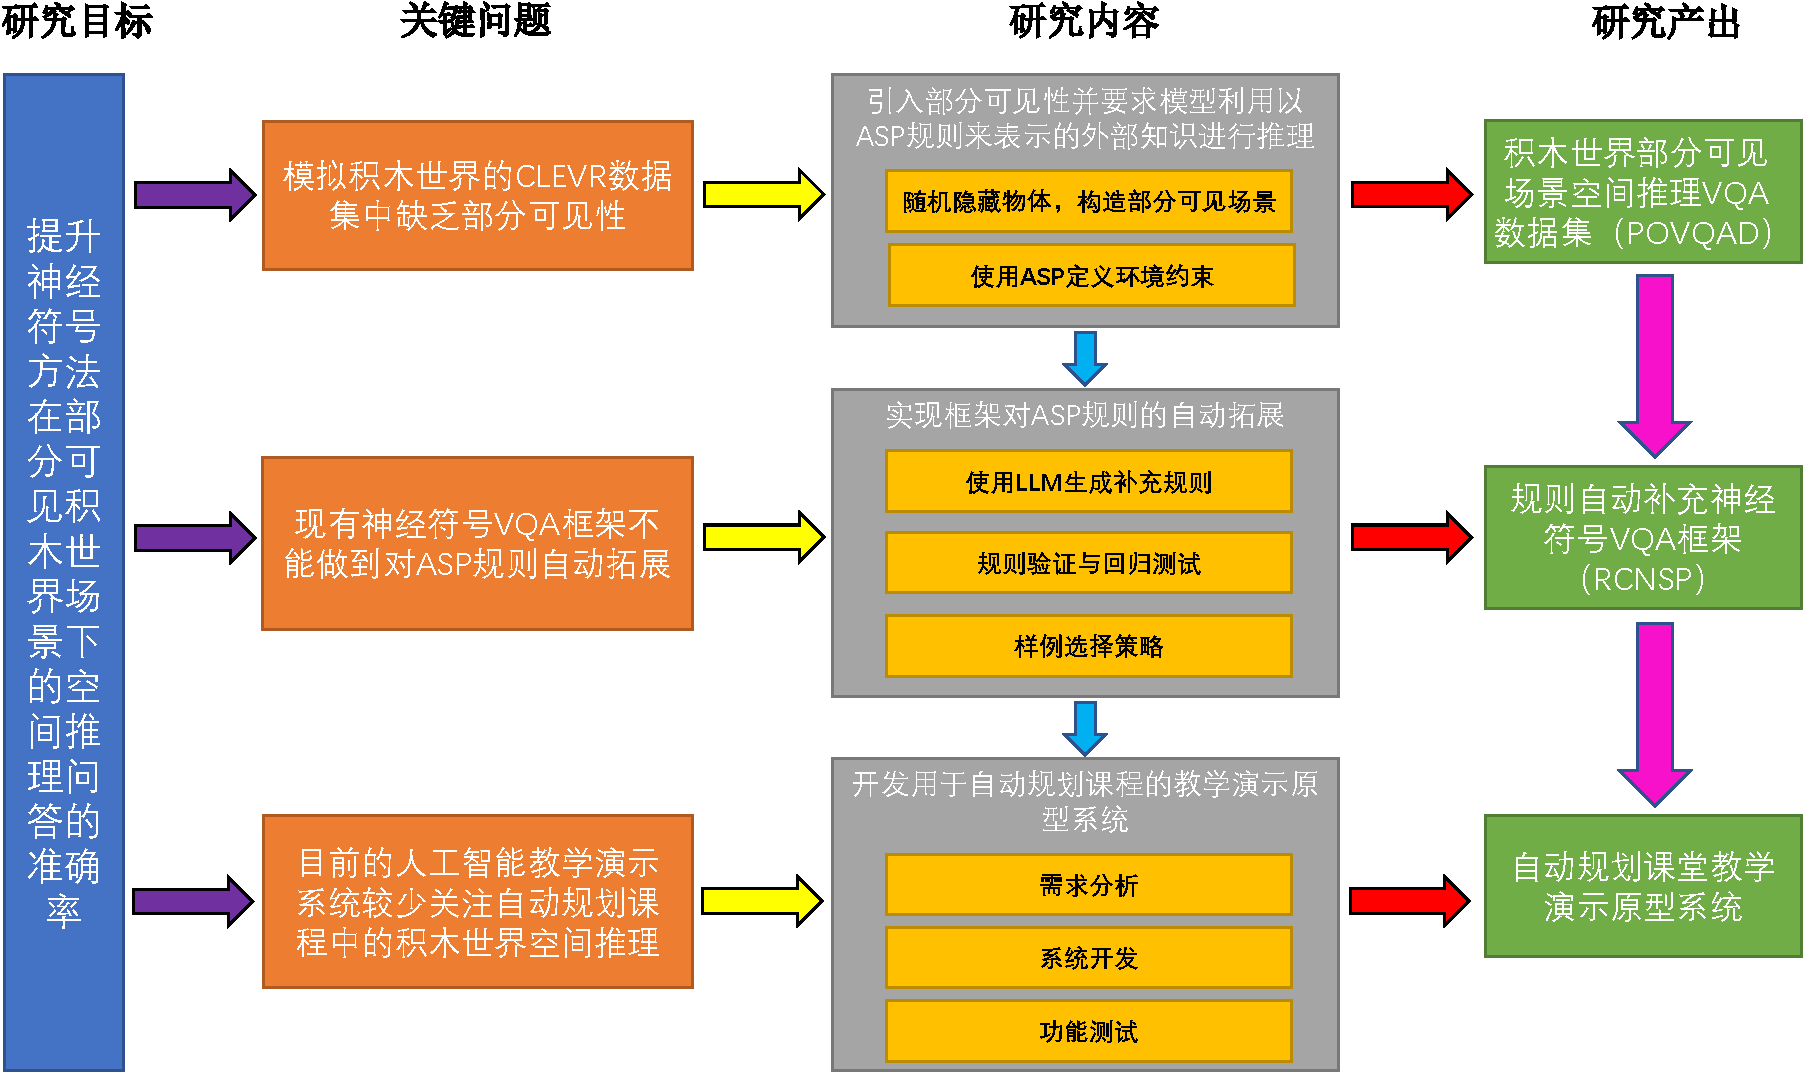
\includegraphics[width=\textwidth]{figures/research-guideline-crop.pdf}
    \caption{研究计划}
    \label{plan}
\end{figure}
% \begin{figure}[h]
%     \centering
%     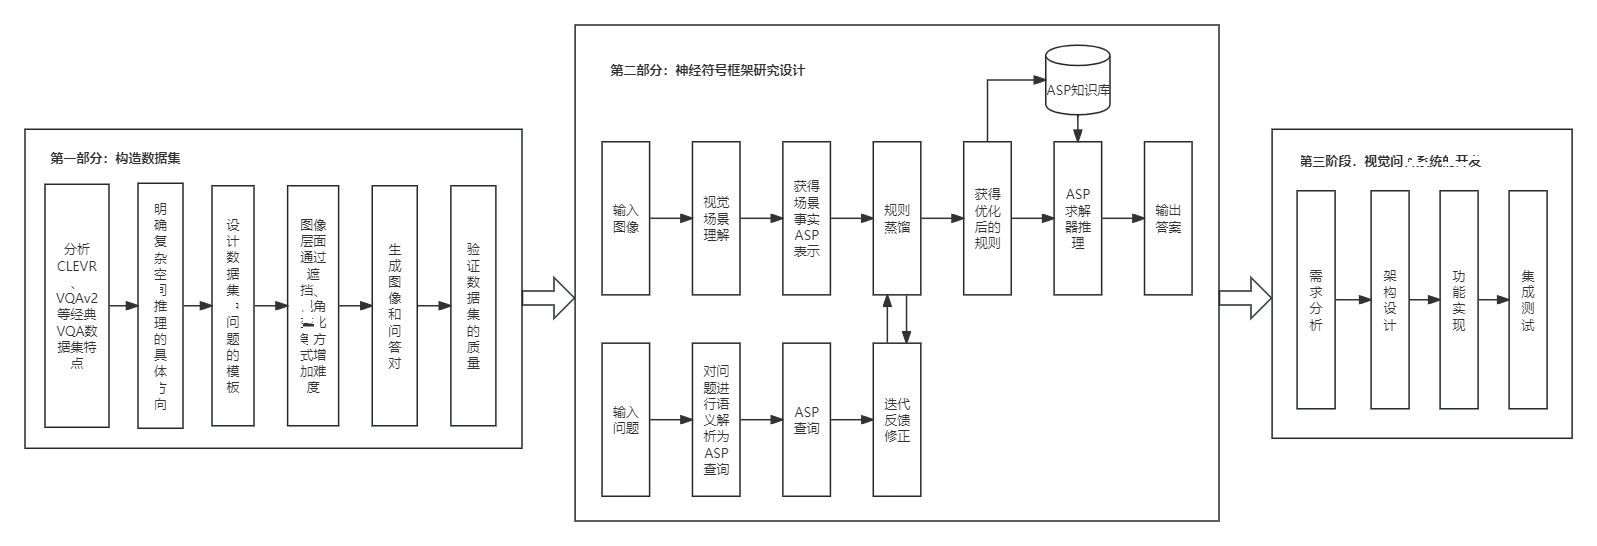
\includegraphics[width=\textwidth]{process.png}
%     \caption{技术路线图}
%     \label{roadmap}
% \end{figure}
\section{论文结构}
本文共分为六个章节,各章节的主要内容具体如下:

第一章为绪论,总体介绍本文的研究背景及意义、相关研究现状、研究思路及本文的结构安排。

第二章为背景知识,对本文涉及到的主要技术进行介绍,具体包括CLEVR数据集、ASP程序语法及ASP求解器、
GLIP以及DSPy。

第三章为数据集构建。对本文所用的视觉问答数据集进行详细介绍,
包括数据集的构造目的、数据集的研究方向、数据集的设计流程以及对数据集质量的验证。

第四章为神经符号VQA框架的研究设计。本章详细介绍本文设计的神经符号VQA框架,
包括总体架构、视觉场景理解、语义解析、知识蒸馏、迭代反馈、规则修正和 ASP 推理等模块,并通过对比试验证明了相比于VLM直接问答,神经符号方法能够有效提升模型在部分可见场景
下回答空间推理问题的正确率,并证明了本文新增的知识蒸馏模块能够进一步提升神经符号方法解决空间推理任务时的性能。

第五章为问答系统的设计与实现。对本文设计的VQA课堂教学演示原型系统进行详细介绍
,包括系统需求分析、系统架构设计、模块划分、模块实现和系统集成等内容。

第六章中对本文工作加以总结,分析本文的创新点和不足之处,并对未来的研究方向进行展望。
